\documentclass[letterpaper,12pt]{article}

\usepackage[top=1in, left=1.25in, right=1.25in, bottom=1in]{geometry}
\usepackage[utf8]{inputenc}
\usepackage[T1]{fontenc}
\usepackage[spanish]{babel}
\usepackage{graphicx}
\usepackage{caption}
\usepackage{float}
\usepackage[backend=biber,style=numeric,sorting=none]{biblatex}
\addbibresource{bib/referencias.bib}

\begin{document}

\tableofcontents
\clearpage

\section{Introducción}

\begin{itemize}
\item \textbf{Planteamiento del Problema:} En esta práctica se busca resolver 3 ejercicios matemáticos de manera recursiva: Factorial, serie de Fibbonacci y Conjetura de Collatz, implementandolos en un menú de opciones en Java.

\item \textbf{Motivación:} Con esta práctica se busca entender la resolución de problemas recursivos desde sus casos base, asegurándonos que cada función se ejecute adecuadamente, y una correcta implementación de un menú en Java interactivo con el usuario.

\item \textbf{Objetivos:} Comprender la recursividad en Java, validando el funcionamiento correcto de cada función mediante entradas y salidas, así como la implementación de la resolución de los problemas en un menú de opciones iterativo.

\end{itemize}
\section{Marco Teórico}
\textbf{Factorial:} Es el producto de todos los números enteros positivos desde 1 hasta ese número n. Su representación matemática es: n! = n * (n-1)! ~\cite{factorial}


\textbf{Serie de Fibonacci:} Es una serie de números en la que cada número es una suma de los dos anteriores, empezando siempre ésta en 0 y 1 y terminando en n. Su representación matemática es: F(n) = F(n-1) + F(n-2).~\cite{fibonacci}


\textbf{Conjetura de Collatz:} Es un algoritmo que asegura que todo número entero positivo siempre llegara a 1 mediante la recursión de dos casos, su representación matemática es: f(n) = n/2 si n es par ; 3n + 1 si n es impar~\cite{collatz}

\section{Desarrollo}

\textbf{Solución teórica de los ejercicios:}

Para los tres ejercicios realizados, empezamos planteando la parte teórica, buscando el caso base y después la operación que va a permitir que la función realice lo requerido y de forma recursiva. 
\begin{enumerate}

    \item \textbf{Factorial}

    El caso base del factorial, es cuando \textbf{n} es igual a \textbf{1}, la fórmula del factorial es \textbf{n(n-1)}, entonces en el código, se rompe la recursividad cuando el número es igual a 1, y cuando no lo es, se regresa el número multiplicado por la misma función factorial pero disminuido en 1.

    \item \textbf{Serie de Fibonacci}

    En fibonacci los casos base son cuando \textbf{n} es igual a \textbf{0} ó \textbf{1}. Para que la función haga lo que queremos, necesitamos sumar el numero anterior con el número anterior a ese hasta llegar al caso base, y es lo que hacemos en el código, si no se rompe la recursividad, se hace la suma de los dos números anteriores hasta que la recursividad se rompa.  

    \item \textbf{Conjetura de Collatz}

    En la Conjetura de Collatz se realiza una evaluación dentro de la función para determinar si es par o impar y realizar su correspondiente operación; si \textbf{n} es par se divide entre 2 \textbf{(n/2)} y se llama de nuevo a la función de forma recursiva, en caso de ser \textbf{n} impar se multiplica por 3 y se suma 1 \textbf{(n*3+1)}, pero siempre evaluando si se llegó al caso base; el caso base es llegar al \textbf{1}, pero anteriormente a este número entra al ciclo infinito del \textbf{4,2,1,4,2,1...}, por ello es necesario cerrar ese ciclo con el \textbf{1}.

    \item \textbf {Desarrollo del menú:}
            
    Se realizó el código de un menú interactivo de opciones en Java, utilizando para ello una variable \textbf{''opcion''} que determine la elección del usuario, y haciendo uso de \textbf{switch case} para crear el menú. Utilizando un \textbf{do-while} para que el menú se mantenga ejecutándose mientras el usuario no decida salir del programa, de tal forma que puede hacer uso de todas las opciones del menú en una sola ejecución.
    
    Por último, integramos los métodos en el menú, ajustando los casos en el orden requerido, poniendo primero el factorial, después la serie de Fibonacci y terminando con la conjetura de Collatz. Agregamos también algunas impresiones para cada caso con el objetivo de dar una buena presentación e imprimir los resultados de los métodos. Además de agregar los Scanners necesarios para pedir un número al usuario, y así, hacer ejecución de las opciones.

    Al seleccionar la opción 4, se rompe el ciclo \textbf{do-while}, por lo que se termina la ejecución del programa.

    \end{enumerate}

\section{Resultados}

\begin{figure}[H]
    \centering
    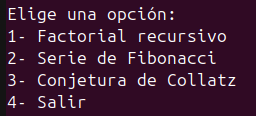
\includegraphics[width=12cm]{Imagenes/Menu.png}
    \caption*{Todas las funciones integradas en un solo menú}
\end{figure}

\begin{figure}[H]
    \centering
    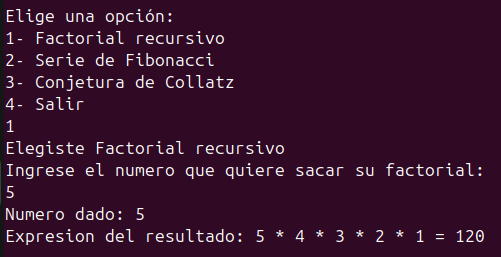
\includegraphics[width=15cm]{Imagenes/Factorial.png}
    \caption*{\centering Opción 1, mostrando el factorial de un número ingresado y la operación que se realizó}
\end{figure}

\begin{figure}[H]
    \centering
    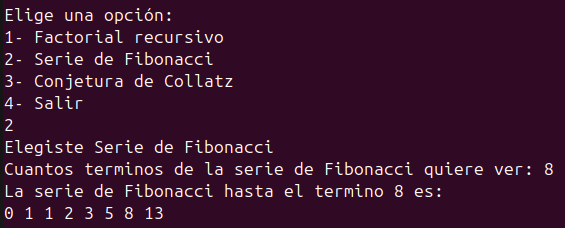
\includegraphics[width=15cm]{Imagenes/Fibonacci.png}
    \caption*{\centering Opción 2, mostrando la serie de Fibonacci con los términos que el usuario solicitó}
\end{figure}

\begin{figure}[H]
    \centering
    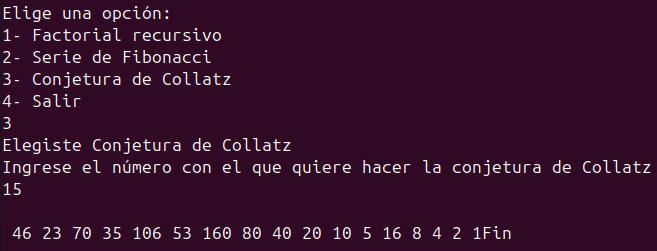
\includegraphics[width=15cm]{Imagenes/Collatz.png}
    \caption*{\centering Opción 3, mostrando los resultados de las operaciones que realiza la conjetura}
\end{figure}

\begin{figure}[H]
    \centering
    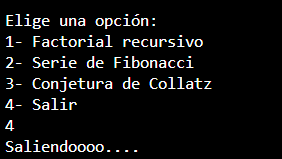
\includegraphics[width=15cm]{Imagenes/saliendo.png}
    \caption*{\centering Opción 4, saliendo de la ejecución del programa}
\end{figure}

\section{Conclusiones}
Se logró una implementación correcta de un menú iterativo, que permite ejecutar los 3 problemas recursivos; así como comprender la importancia de identificar y definir correctamente los casos base para su solución, ademas de validar las entradas y salidas, para un funcionamiento correcto en cada problema.


\clearpage

\printbibliography

\clearpage

\section{Reto para token}
El triángulo de Pascal es una matriz de forma triangular, la cuál en cada una de sus filas empiezan y terminan en uno, y los dígitos son la suma de los dos dígitos encima de él.

Para manejar el triángulo de pascal en código, nos ayudamos usando el triángulo con 2 posiciones, una que mida las filas o pisos, y otra que mida las posiciones dentro del triángulo.

\begin{figure}[H]
    \centering
    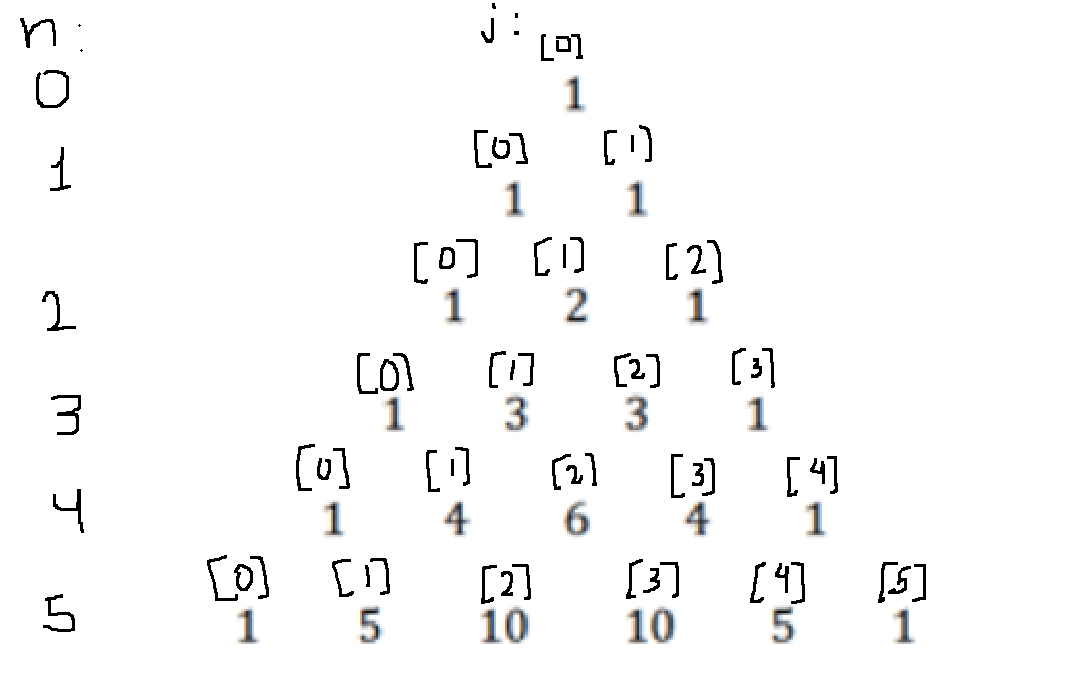
\includegraphics[width=15cm]{Imagenes/ejemplo.png}
    \caption*{\centering Forma gráfica de entender el código del Triángulo de Pascal}
\end{figure}

El caso base del triángulo de pascal es cuando llegamos a los bordes del triángulo, donde en esos casos siempre es uno, y si no se cumple el caso base, se hace la suma de la posición de \textbf{(n-1, j-1)} y \textbf{(n-1, j)}, lo que significa que hace la suma de los dos números que están en el piso de arriba justo encima del número a calcular.

\clearpage

Usamos una función recursiva, y lo que hace es calcular el número en la posición de \textbf{n} y \textbf{j} que es ingresada, usando la lógica explicada anteriormente, y para que se imprima la pirámide completa, usamos 2 ciclos \textbf{for} anidados que van iterando en las posiciones de la pirámide y calculando todos los números.

Usamos otro ciclo \textbf{for} que va imprimiendo espacios según el nivel en el que está para que la pirámide sí tenga forma de pirámide.

\begin{figure}[H]
    \centering
    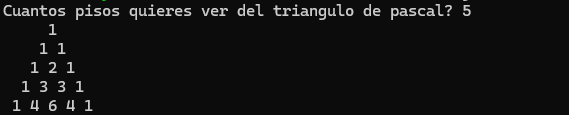
\includegraphics[width=15cm]{Imagenes/pascal.png}
    \caption*{\centering Código ejecutado}
\end{figure}

\end{document}